\documentclass[demo, 12pt, notitlepage, letterpaper]{report}
\usepackage[version=4]{mhchem}
\usepackage{siunitx}
\usepackage[margin=1in]{geometry}
\usepackage{tabularx}
\usepackage{ragged2e}
\usepackage[font=small]{caption}
\usepackage{calculator}
\usepackage{luacode}
\usepackage{pythontex}

\DeclareSIUnit\ml{\milli\litre}
\DeclareSIUnit\mpl{\mol\per\litre}
\DeclareSIUnit\mmol{\milli\mole}
\DeclareSIUnit\gpl{\gram\per\mol}
\DeclareSIUnit\kjpmol{\kilo\joule\per\mol}
\DeclareSIUnit\heatcap{\joule\per\celsius\per\gram}

\sisetup{space-before-unit = true, free-standing-units = true}

\title{Thermokinetics Lab}
\author{Leon Si}
\date{February 22, 2022}

\begin{document}
\maketitle

% Rubric:
% Sufficient relevant quantitative and qualitative raw data supports a detailed and valid research question conclusion.
% Appropriate and sufficient data processing is carried out with the accuracy required to validate conclusion; fully consistent with the experimental data.
% Full and appropriate consideration of the impact of measurement uncertainty on the analysis.
% Processed data correctly interpreted so that a completely valid and detailed conclusion to the research question can be deduced.

\section*{Data}

% \begin{noindent}
\begin{pycode}
"""
[0]: Volume of CuSO4 Time of Zn Addition
[1]: Initial temp
[2]: Time of Zn addition
[3]: b value for equation of cooling line
[4]: m value for equation of cooling line (could be positive/negative)
[5]: R value of cooling line
"""

data = [
	# Eric, Bobby, Bryan	20	24.4	72	75.358 - 0.0417x	-0.9918
	[20, 24.4, 72, 75.358, -0.0417, -0.9918],
	# Estelle, Hannah, Molly 	20	24.2	132	76.057 - 0.0521x	-0.9591
	[20, 24.2, 132, 76.1, -0.0521, -0.9591],
	# Lily, Cindy, Devanshi	20	24.2	60	74.909-0.086299x	-0.99338
	[20, 24.2, 60, 74.9, -0.086299, -0.99338],
	# Kevin, Leon, Thomas	20	24.8	72	38.948 - 0.0052021x	-0.95144
	[20, 24.8, 72, 38.948, -0.0052021, -0.95144],
	# Avaneesh, Artin, Ethan, Yucen	20	24.6	96	75.883 - 2.5313x	-0.99564
	[20, 24.6, 96, 75.883, -2.5313 / 60, -0.99564], # time of cooling line was given in minutes
	# Colin, Henry, Collin, Ishan	20	23.1	14	35.707+0.0060035x	0.952365476
	[20, 23.1, 14, 35.707, 0.0060035, 0.952365476],
	# Jasmine, Amy, Tina	20	23.8	15	74.526-0.059536x	-0.8973
	[20, 23.8, 15, 74.526, -0.059536, -0.8973],
	# Prachi, Michelle, Naina 	20	24.6	96	61.881 - 0.02918	-0.99694
	[20, 24.6, 96, 61.881, -0.02918, -0.99694],
]

def get_data_row(row_index: int):
	# Three sig fig
	def tsf(num):
		return '%s' % float('%.3g' % num)

	row = data[row_index]
	sign = "+" if row[4] > 0 else "-"
	equation = f"{row[3]:.3g} {sign} {abs(row[4]):.3g}$x$"

	return f"""
		{row_index}
		& {row[0]}
		& {row[1]}
		& {row[2]}
		& {equation}
		& {tsf(row[5])}
	"""
\end{pycode}
% \end{noindent}

\begin{table}[hbt!]
	\caption{Data collected from 8 trials of the experiment. Equation of cooling line approximates the temperature of the solution in Celsius at $x$ seconds. The parameters are rounded to 3 significant figures.}
	\def\arraystretch{1.5}
	\begin{tabularx}{\linewidth}{|
			>{\RaggedRight}X|
			>{\RaggedRight}X|
			>{\RaggedRight}X|
			>{\RaggedRight}X|
			>{\RaggedRight}X|
			>{\RaggedRight}X|
		}
		\hline
		Trial \#
		 & Volume of \ce{CuSO4} /\ml
		 & Baseline temperature /\celsius
		 & Time of \ce{Zn} addition /\second
		 & Equation of cooling line
		 & R value
		\\\hline
		\py{get_data_row(0)}
		\\\hline
		\py{get_data_row(1)}
		\\\hline
		\py{get_data_row(2)}
		\\\hline
		\py{get_data_row(3)}
		\\\hline
		\py{get_data_row(4)}
		\\\hline
		\py{get_data_row(5)}
		\\\hline
		\py{get_data_row(6)}
		\\\hline
		\py{get_data_row(7)}
		\\\hline
	\end{tabularx}
\end{table}

\section*{Analysis}

The data in Table 1 can be used to find the molar enthalpy of formation of \ce{ZnSO4}. For the following calculations, the values in Trial 4 are used.

To find the molar enthalpy of formation of \ce{ZnSO4}, the energy change of the reaction $Q_{reaction}$ and the moles of \ce{ZnSO4} ($n_{ZnSO4}$) must be known.

To find the moles of \ce{ZnSO4} produced, the moles of \ce{CuSO4} must be knonwn. Using the known concentration of \ce{CuSO4} (1\mpl), the volume of \ce{CuSO4} can be converted to moles of \ce{CuSO4}:
\begin{align*}
	c     & = \frac{n}{V}        \\
	1\mpl & = \frac{n}{20\ml}    \\
	n     & = 20\mmol~\ce{CuSO4}
\end{align*}

Then, to find the moles of \ce{ZnSO4}, the balanced chemical equation of the reaction between zinc metal (\ce{Zn}) and aqueous copper sulfate (\ce{CuSO4}) is used:

\centerline{\ce{CuSO4_{(aq)} + Zn_{(s)} -> ZnSO4_{(aq)} + Cu_{(s)}}}

This equation gives the mole ratio between \ce{CuSO4} and \ce{ZnSO4}, which can be used to find the moles of \ce{ZnSO4} produced in the reaction:
\begin{align*}
	n_{\ce{ZnSO4}} & = 20\mmol~\ce{CuSO4} * \frac{1\mol~{\ce{ZnSO4}}}{1\mol~{\ce{CuSO4}}} = 20\mmol~{\ce{ZnSO4}}
\end{align*}

In addition to the number of moles of \ce{ZnSO4}, the change in energy of the reaction ($Q_{reaction}$) must also be known. The energy lost by the reaction is equal to the energy gained by the solution: $Q_{reaction} = -Q_{solution}$. To find $Q_{solution}$, the mass $m$ of the solution, the specific heat capacity $c$ of the solution, and the temperature change $\Delta T$ of the solution are all needed.

Since the solution is dilute, the mass of the solution can be approximated using the density of water, 1~\unit{\gram\per\cm}. Thus, the mass of the solution is:
\begin{align*}
	m & = \rho * V                      \\
	m & = 1~\unit{\gram\per\cm} * 20\ml \\
	m & = 20\gram
\end{align*}

The heat capacity of the solution is approximated with the specific heat capacity of water (4.184\heatcap). Thus, $c = 4.184\heatcap$

To calculate the change in temperature of the solution, the initial and final temperatures are needed. The initial temperature of the solution before the reaction ($T_i$) is equal to the \textit{Baseline temperature} column in Table 1.

To obtain the final temperature of the solution, the cooling of the solution needs to be taken into account. This is done by plugging in the time when \ce{Zn} was added into the solution into the equation of the cooling line.
\begin{align*}
	T_f & = 38.948 - 0.0052021x    \\
	T_f & = 38.948 - 0.0052021(72) \\
	T_f & = 38.5734488\celsius
\end{align*}

This value represents the point $x$ in the following graph:

\centerline{\noindent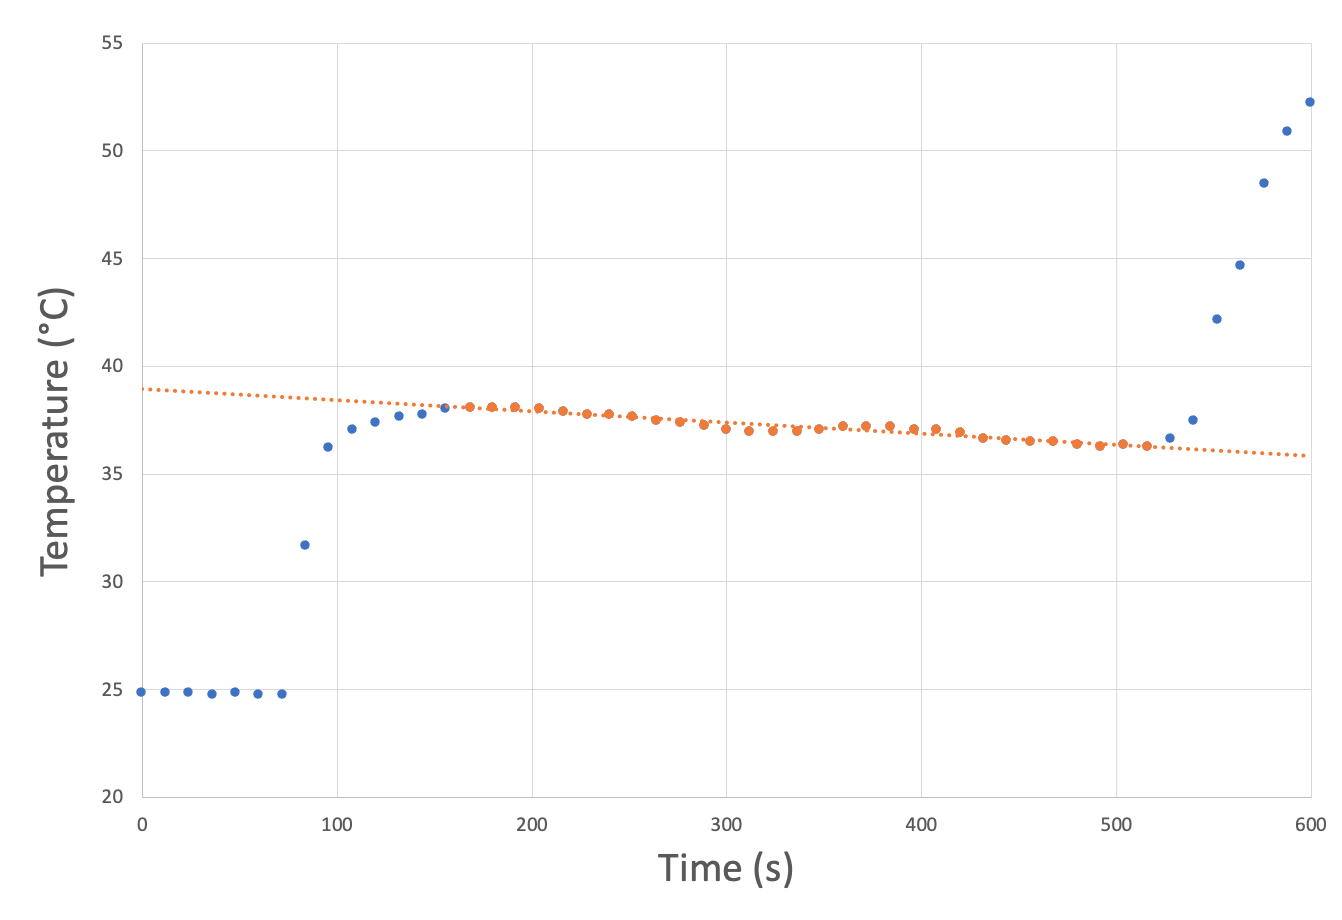
\includegraphics{time-vs-temperature.png}}


With these values, the energy change of the solution and the energy change of the reaction can be determined:
\begin{align*}
	Q_{solution} & = mc\Delta T = mc(T_f - T_i)
	\\
	Q_{solution} & = (20\gram) * (4.184\heatcap) * (38.5734\celsius - 24.8\celsius)
	\\
	Q_{solution} & = 1152.56\joule
	\\
	Q_{reaction} & = -Q_{solution}
	\\
	Q_{reaction} & = -1152.56\joule
\end{align*}

Finally, the molar enthalpy of the reaction can be calculated:
\begin{align*}
	\Delta H_{reaction} & = \frac{Q_{reaction}}{n}                        \\
	\Delta H_{reaction} & = \frac{-1152.56\joule}{0.02\mol}               \\
	\Delta H_{reaction} & = -57628~\unit{\joule\per\mol} = -57.628\kjpmol
\end{align*}

Performing the above calculation for all trials gives the following table of values:

% \begin{noindent}
\begin{luacode*}
	--[[
			[1] = Volume of CuSO4 Time of Zn Addition
			[2] = Initial temp
			[3] = Time of Zn addition
			[4] = b value for equation of cooling line
			[5] = m value for equation of cooling line (could be positive/negative)
		]]
	data = {
		-- Eric, Bobby, Bryan	20	24.4	72	75.358 - 0.0417x	-0.9918
		{20, 24.4, 72, 75.358, -0.0417},
		-- Estelle, Hannah, Molly 	20	24.2	132	76.057 - 0.0521x	-0.9591
		{20, 24.2, 132, 76.1, -0.0521},
		-- Lily, Cindy, Devanshi	20	24.2	60	74.909-0.086299x	-0.99338
		{20, 24.2, 60, 74.9, -0.086299},
		-- Kevin, Leon, Thomas	20	24.8	72	38.948 - 0.0052021x	-0.95144
		{20, 24.8, 72, 38.948, -0.0052021},
		-- Avaneesh, Artin, Ethan, Yucen	20	24.6	96	75.883 - 2.5313x	-0.99564
		{20, 24.6, 96, 75.883, -2.5313},
		-- Colin, Henry, Collin, Ishan	20	23.1	14	35.707+0.0060035x	0.952365476
		{20, 23.1, 14, 35.707, 0.0060035},
		-- Jasmine, Amy, Tina	20	23.8	15	74.526-0.059536x	-0.8973
		{20, 23.8, 15, 74.526, -0.059536},
		-- Prachi, Michelle, Naina 	20	24.6	96	61.881 - 0.02918	-0.99694
		{20, 24.6, 96, 61.881, -0.02918},
	}

	function qreaction(t_initial, t_final)
	m = 20
	c = 4.184

	q = m * c * (t_final - t_initial)

	tex.sprint(("%.4g"):format(-q))
	end

	function hreaction(t_initial, t_final)
	m = 20
	c = 4.184

	q = m * c * (t_final - t_initial)

	mols = 0.02
	h = -q / mols / 1000 -- *k*J/mol

	-- Three significant figures
	tex.sprint(("%.3g"):format(h))
	end
\end{luacode*}
% \end{noindent}

\newcounter{hreactionrownumber}
\setcounter{hreactionrownumber}{0}
\newcommand{\hreactionrow}[5]{%
	% #1: Baseline temperature
	% #2: Time of Zn addition
	% #3: b parameter of equation of cooling line
	% #4: sign of m
	% #5: m parameter of equation of cooling line
	\addtocounter{hreactionrownumber}{1}
	\thehreactionrownumber
	&
	\luaexec{tex.sprint(("\%.3g"):format(#3 #4 #5 * #2))}
	&
	\directlua{qreaction(#1, #3 #4 #5 * #2)}
	&
	\directlua{hreaction(#1, #3 #4 #5 * #2)}
}

\begin{table}[hbt!]
	\caption{Calculations of $\Delta H_{reaction}$ for all trials.}
	\def\arraystretch{1.5}
	\begin{tabularx}{\linewidth}{|
			p{0.1\linewidth}|
			p{0.3\linewidth}|
			>{\RaggedRight}X|
			>{\RaggedRight}X|
		}
		\hline
		Trial \#
		 & Final Temperature $T_f$ /\unit{\celsius}
		 & $Q_{reaction}$ /\unit{\joule\per\mol}
		 & $\Delta H_{reaction}$ /\unit{\kjpmol}
		\\\hline
		% Eric, Bobby, Bryan	20	24.4	72	75.358 - 0.0417x	-0.9918
		\hreactionrow{24.4}{72}{75.358}{-}{0.0417}
		\\\hline
		% Estelle, Hannah, Molly 	20	24.2	132	76.057 - 0.0521x	-0.9591
		\hreactionrow{24.2}{132}{76.057}{-}{0.0521}
		\\\hline
		% Lily, Cindy, Devanshi	20	24.2	60	74.909-0.086299x	-0.99338
		\hreactionrow{24.2}{60}{74.909}{-}{0.086299}
		\\\hline
		% Kevin, Leon, Thomas	20	24.8	72	38.948 - 0.0052021x	-0.95144
		\hreactionrow{24.8}{72}{38.948}{-}{0.0052021}
		\\\hline
		% Avaneesh, Artin, Ethan, Yucen	20	24.6	96	75.883 - 2.5313x	-0.99564
		\hreactionrow{24.6}{96}{75.883}{-}{0.0422}
		\\\hline
		% Colin, Henry, Collin, Ishan	20	23.1	14	35.707+0.0060035x	0.952365476
		\hreactionrow{23.1}{14}{35.707}{-}{0.0060035}
		\\\hline
		% Jasmine, Amy, Tina	20	23.8	15	74.526-0.059536x	-0.8973
		\hreactionrow{23.8}{15}{74.526}{-}{0.059536}
		\\\hline
		% Prachi, Michelle, Naina 	20	24.6	96	61.881 - 0.02918	-0.99694
		\hreactionrow{24.6}{96}{61.881}{-}{0.02918}
		\\\hline
	\end{tabularx}
\end{table}

Thus, the experimental value for $\Delta H_{reaction}$ can be determined by taking the average of the values from all 8 trials. The uncertainty can be calculated using the half-range method:

\begin{align*}
	\Delta H_{reaction} & = \frac{-201 + -188 + -191 + -57.6 + -198 + -52.4 + -209 + -144}{8}
	\Delta H_{reaction} & =
\end{align*}

\subsection*{Comparison with Theoretical Value}
To find the theoretical value of this reaction, the following formula is used:

\begin{align*}
	\Delta H_{reaction} = \sum \Delta {H_f}_{products} - \sum \Delta {H_f}_{reactants}
\end{align*}

According to NIST, the molar enthalpy formation of \ce{CuSO4} is -769.98\kjpmol and the molar enthalpy of formation of \ce{ZnSO4} is -980.14\kjpmol . Because \ce{Zn} and \ce{Cu} are in their standard states, the molar enthalpy of \ce{Zn} and \ce{Cu} is 0\kjpmol .
\begin{align*}
	\Delta H_{reaction} & = -980.14\kjpmol - (-769.98\kjpmol) \\
	\Delta H_{reaction} & = -210.16\kjpmol
\end{align*}

% Presentation of the investigation is clear. Errors do not hamper understanding of the focus, process and outcomes.
% Clear report structure; necessary information on focus, process and outcomes is present and presented coherently.
% Report is relevant and concise; facilitates a ready understanding of the focus, process and outcomes.
% Subject specific terminology and conventions is appropriate and correct. Errors do not hamper understanding.
\end{document}

% Performing the above calculation for the values in each trial yields the following table of values:

% \newcommand{\finaltemprow}[3]{%
% 	% #1: Time of Zn addition
% 	% #2: b value in cooling line equation
% 	% #3: m value in cooling line equation
% 	\addtocounter{temprownumber}{1}
% 	\thetemprownumber
% 	& #1
% 	& #2 - #3$x$
% 	& \luaexec{tex.sprint(("\%.3g"):format(#2-#3*#1))}
% }
% \newcommand{\finaltemprowpos}[3]{%
% 	% #1: Time of Zn addition
% 	% #2: b value in cooling line equation
% 	% #3: m value in cooling line equation
% 	\addtocounter{temprownumber}{1}
% 	\thetemprownumber
% 	& #1
% 	& #2 + #3$x$
% 	& \luaexec{tex.sprint(("\%.3g"):format(#2+#3*#1))}
% }

% \begin{table}[hbt!]
% 	\caption{Final temperature of the solution calculated for each trial.}
% 	\def\arraystretch{1.5}
% 	\begin{tabularx}{\linewidth}{|
% 			>{\RaggedRight}X|
% 			>{\RaggedRight}X|
% 			>{\RaggedRight}X|
% 			>{\RaggedRight}X|
% 		}
% 		\hline
% 		Trial \#
% 		 & Time of Zn addition /\unit{\second}
% 		 & Equation of cooling line
% 		 & Final temperature /\unit{\celsius}
% 		\\\hline
% 		% Eric, Bobby, Bryan	20	24.4	72	75.358 - 0.0417x	-0.9918
% 		\finaltemprow{72}{75.4}{0.0417}
% 		\\\hline
% 		% Estelle, Hannah, Molly 	20	24.2	132	76.057 - 0.0521x	-0.9591
% 		\finaltemprow{132}{76.1}{0.0521}
% 		\\\hline
% 		% Lily, Cindy, Devanshi	20	24.2	60	74.909-0.086299x	-0.99338
% 		\finaltemprow{60}{74.9}{0.0863}
% 		\\\hline
% 		% Kevin, Leon, Thomas	20	24.8	72	38.948 - 0.0052021x	-0.95144
% 		\finaltemprow{72}{38.9}{0.00520}
% 		\\\hline
% 		% Avaneesh, Artin, Ethan, Yucen	20	24.6	96	75.883 - 2.5313x	-0.99564
% 		\finaltemprow{96}{75.9}{0.0422}
% 		\\\hline
% 		% Colin, Henry, Collin, Ishan	20	23.1	14	35.707+0.0060035x	0.952365476
% 		\finaltemprowpos{14}{35.7}{0.00600}
% 		\\\hline
% 		% Jasmine, Amy, Tina	20	23.8	15	74.526-0.059536x	-0.8973
% 		\finaltemprow{15}{74.5}{0.0595}
% 		\\\hline
% 		% Prachi, Michelle, Naina 	20	24.6	96	61.881 - 0.02918	-0.99694
% 		\finaltemprow{96}{61.9}{0.0292}
% 		\\\hline
% 	\end{tabularx}
% \end{table}